\documentclass[11pt,a4paper]{article}

% Packages
\usepackage{amsmath}
\usepackage{amssymb}
\usepackage{amsthm}
\usepackage[margin=1in]{geometry}
\usepackage{enumitem}
\usepackage{tikz}
\usepackage{pgfplots}
\usepackage{xcolor}
\pgfplotsset{compat=1.18}

% Custom commands
\newcommand{\stage}[1]{\textbf{\textcolor{blue}{#1}}}

% Title information
\title{Exercise Sheet 3: Bifurcations\\
Question 3 - Complete Solution}
\author{Methods of Applied Mathematics}
\date{}

\begin{document}

\maketitle

\section*{Problem Statement}

Consider the dynamical system:
\begin{align*}
\dot{x} &= y - 3x \\
\dot{y} &= \alpha x - x^2
\end{align*}
for $-9/4 < \alpha < 9/4$.

\textbf{Tasks:}
\begin{enumerate}[label=(\alph*)]
\item Compute and classify the stability/type of any equilibria
\item What bifurcation happens in the system at $\alpha = 0$?
\item Draw a bifurcation diagram with $\alpha$ on the horizontal axis, and $x$ on the vertical. What would the diagram look like if you drew $\alpha$ against $y$?
\end{enumerate}

\vspace{10pt}
\hrule
\vspace{10pt}

\section{Step 1: Find Equilibria}

\subsection*{Set up equilibrium conditions}

For equilibria, we require $\dot{x} = 0$ and $\dot{y} = 0$ simultaneously:
\begin{align*}
y - 3x &= 0 \quad \Rightarrow \quad y = 3x \\
\alpha x - x^2 &= 0 \quad \Rightarrow \quad x(\alpha - x) = 0
\end{align*}

\subsection*{Solve for equilibrium points}

From the second equation: either $x = 0$ or $x = \alpha$

\textbf{Equilibrium 1:} $x = 0$
\[
y = 3(0) = 0 \quad \Rightarrow \quad \boxed{(x^*, y^*) = (0, 0)}
\]

\textbf{Equilibrium 2:} $x = \alpha$
\[
y = 3\alpha \quad \Rightarrow \quad \boxed{(x^*, y^*) = (\alpha, 3\alpha)}
\]

\subsection*{Special case: $\alpha = 0$}

When $\alpha = 0$: both equilibria coincide at $(0, 0)$

\subsection*{XYZ Analysis of Equilibrium Structure}

\begin{itemize}[leftmargin=*]
\item \stage{STAGE X (What we found):} Two equilibria for $\alpha \neq 0$: one pinned at the origin, one that moves linearly with $\alpha$ along the line $y = 3x$. They collide at the origin when $\alpha = 0$.

\item \stage{STAGE Y (Why this structure):} The equation $\dot{y} = \alpha x - x^2 = x(\alpha - x)$ factors, giving two roots. The constraint $y = 3x$ from the first equation means equilibria must lie on this line in the phase plane. As $\alpha$ varies:
\begin{itemize}
\item The origin $(0,0)$ is always an equilibrium (pinned)
\item The second equilibrium $(\alpha, 3\alpha)$ moves along $y = 3x$:
  \begin{itemize}
  \item For $\alpha < 0$: in third quadrant (left and below origin)
  \item For $\alpha = 0$: at origin (collision)
  \item For $\alpha > 0$: in first quadrant (right and above origin)
  \end{itemize}
\end{itemize}

\item \stage{STAGE Z (What this means):} One equilibrium passing through another pinned equilibrium is the signature of a transcritical bifurcation. The collision at $\alpha = 0$ will involve an exchange of stability.
\end{itemize}

\vspace{10pt}
\hrule
\vspace{10pt}

\section{Step 2: Compute Jacobian Matrix}

\subsection*{General Jacobian}

For the system $\dot{x} = f(x,y)$, $\dot{y} = g(x,y)$:
\[
J = \begin{pmatrix}
\frac{\partial f}{\partial x} & \frac{\partial f}{\partial y} \\[5pt]
\frac{\partial g}{\partial x} & \frac{\partial g}{\partial y}
\end{pmatrix}
\]

With $f(x,y) = y - 3x$ and $g(x,y) = \alpha x - x^2$:
\[
J = \begin{pmatrix}
-3 & 1 \\
\alpha - 2x & 0
\end{pmatrix}
\]

\subsection*{XYZ Analysis of Jacobian}

\begin{itemize}[leftmargin=*]
\item \stage{STAGE X (What we have):} The Jacobian is simple - constant entries except for $\alpha - 2x$ in the lower-left, which depends on both the parameter and equilibrium location.

\item \stage{STAGE Y (Why this form):} The partial derivatives are:
\begin{itemize}
\item $\partial f/\partial x = -3$: constant damping in $\dot{x}$ equation
\item $\partial f/\partial y = 1$: linear coupling from $y$ to $\dot{x}$
\item $\partial g/\partial x = \alpha - 2x$: varies with position, reflects the $x(\alpha-x)$ structure
\item $\partial g/\partial y = 0$: no direct $y$-dependence in $\dot{y}$
\end{itemize}
The $\alpha - 2x$ term is crucial: at origin it's $\alpha$, at $(\alpha, 3\alpha)$ it becomes $-\alpha$.

\item \stage{STAGE Z (What this determines):} The eigenvalues of $J$ at each equilibrium will determine stability. The symmetry in how $\alpha$ appears (positive at origin, negative at second equilibrium) suggests stability exchange.
\end{itemize}

\vspace{10pt}
\hrule
\vspace{10pt}

\section{Step 3: Analyze Equilibrium at Origin}

\subsection*{Jacobian at $(0, 0)$}

\[
J(0,0) = \begin{pmatrix}
-3 & 1 \\
\alpha & 0
\end{pmatrix}
\]

\subsection*{Compute trace and determinant}

\begin{align*}
\text{Trace: } \tau &= -3 + 0 = -3 \\
\text{Determinant: } \Delta &= (-3)(0) - (1)(\alpha) = -\alpha
\end{align*}

\subsection*{Find eigenvalues}

Characteristic equation: $\lambda^2 - \tau\lambda + \Delta = 0$
\[
\lambda^2 + 3\lambda - \alpha = 0
\]

Quadratic formula:
\[
\lambda = \frac{-3 \pm \sqrt{9 + 4\alpha}}{2}
\]

\subsection*{Classify by parameter value}

\textbf{Case 1: $\alpha < 0$ (and $\alpha > -9/4$ to keep discriminant real)}

Discriminant: $9 + 4\alpha > 0$ for $\alpha > -9/4$

Both eigenvalues are real. Since:
\begin{itemize}
\item $\Delta = -\alpha > 0$ (product of eigenvalues positive → same sign)
\item $\tau = -3 < 0$ (sum of eigenvalues negative → both negative)
\end{itemize}

\[
\boxed{\text{STABLE NODE}}
\]

Eigenvalues: both negative, real, distinct (for $-9/4 < \alpha < 0$)

\textbf{Case 2: $\alpha = 0$}

\[
\lambda = \frac{-3 \pm 3}{2} \quad \Rightarrow \quad \lambda_1 = 0, \quad \lambda_2 = -3
\]

\[
\boxed{\text{NEUTRAL (one zero eigenvalue)}}
\]

This signals a bifurcation point.

\textbf{Case 3: $\alpha > 0$ (and $\alpha < 9/4$ to stay in given range)}

\begin{itemize}
\item $\Delta = -\alpha < 0$ (product of eigenvalues negative → opposite signs)
\end{itemize}

\[
\boxed{\text{SADDLE POINT}}
\]

Eigenvalues: one positive, one negative, real

\subsection*{XYZ Analysis of Origin Stability}

\begin{itemize}[leftmargin=*]
\item \stage{STAGE X (What we found):} Origin changes from stable node ($\alpha < 0$) through neutral ($\alpha = 0$) to saddle ($\alpha > 0$).

\item \stage{STAGE Y (Why this transition):} The determinant $\Delta = -\alpha$ controls the product of eigenvalues:
\begin{itemize}
\item For $\alpha < 0$: $\Delta > 0$ means eigenvalues have same sign; combined with $\tau < 0$ (negative sum), both must be negative → stable
\item For $\alpha = 0$: $\Delta = 0$ means one eigenvalue is zero → bifurcation
\item For $\alpha > 0$: $\Delta < 0$ means eigenvalues have opposite signs → saddle
\end{itemize}
The trace $\tau = -3$ stays constant (always negative), but the determinant crossing zero at $\alpha = 0$ fundamentally changes the eigenvalue configuration from $(-, -)$ to $(-, +)$.

\item \stage{STAGE Z (What this means physically):} Before bifurcation, the origin is an attractor - all nearby trajectories spiral/flow inward. After bifurcation, it becomes a saddle - trajectories are repelled in one direction (unstable manifold) while attracted in another (stable manifold). The origin loses its basin of attraction.
\end{itemize}

\vspace{10pt}
\hrule
\vspace{10pt}

\section{Step 4: Analyze Equilibrium at $(\alpha, 3\alpha)$}

\subsection*{Existence condition}

This equilibrium only exists for $\alpha \neq 0$ (when $\alpha = 0$, it coincides with origin).

\subsection*{Jacobian at $(\alpha, 3\alpha)$}

\[
J(\alpha, 3\alpha) = \begin{pmatrix}
-3 & 1 \\
\alpha - 2\alpha & 0
\end{pmatrix} = \begin{pmatrix}
-3 & 1 \\
-\alpha & 0
\end{pmatrix}
\]

\subsection*{Compute trace and determinant}

\begin{align*}
\text{Trace: } \tau &= -3 + 0 = -3 \\
\text{Determinant: } \Delta &= (-3)(0) - (1)(-\alpha) = \alpha
\end{align*}

\subsection*{Find eigenvalues}

Characteristic equation:
\[
\lambda^2 + 3\lambda + \alpha = 0
\]

Quadratic formula:
\[
\lambda = \frac{-3 \pm \sqrt{9 - 4\alpha}}{2}
\]

\subsection*{Classify by parameter value}

\textbf{Case 1: $\alpha < 0$}

\begin{itemize}
\item $\Delta = \alpha < 0$ (product negative → opposite signs)
\end{itemize}

\[
\boxed{\text{SADDLE POINT}}
\]

Eigenvalues: one positive, one negative

\textbf{Case 2: $0 < \alpha < 9/4$}

Discriminant: $9 - 4\alpha > 0$ for $\alpha < 9/4$ → real eigenvalues

\begin{itemize}
\item $\Delta = \alpha > 0$ (product positive → same sign)
\item $\tau = -3 < 0$ (sum negative → both negative)
\end{itemize}

\[
\boxed{\text{STABLE NODE}}
\]

Eigenvalues: both negative, real, distinct

\textbf{Note:} At $\alpha = 9/4$, the discriminant vanishes and eigenvalues become complex, but this is outside our detailed analysis.

\subsection*{XYZ Analysis of Moving Equilibrium}

\begin{itemize}[leftmargin=*]
\item \stage{STAGE X (What we found):} The equilibrium $(\alpha, 3\alpha)$ changes from saddle ($\alpha < 0$) to stable node ($\alpha > 0$).

\item \stage{STAGE Y (Why this transition):} The determinant $\Delta = \alpha$ (opposite sign to origin!) controls stability:
\begin{itemize}
\item For $\alpha < 0$: $\Delta < 0$ → saddle (unstable)
\item For $\alpha > 0$: $\Delta > 0$ and $\tau < 0$ → stable node
\end{itemize}
Notice the symmetry with the origin: when origin has $\Delta = -\alpha > 0$ (stable for $\alpha < 0$), this equilibrium has $\Delta = \alpha < 0$ (unstable). When origin has $\Delta = -\alpha < 0$ (saddle for $\alpha > 0$), this equilibrium has $\Delta = \alpha > 0$ (stable). They swap determinant signs, hence swap stability types.

\item \stage{STAGE Z (What this means):} As the moving equilibrium passes through the origin at $\alpha = 0$, it inherits the stability that the origin loses. Before: origin stable, moving point saddle. After: origin saddle, moving point stable. This is the stability exchange characteristic of transcritical bifurcation.
\end{itemize}

\vspace{10pt}
\hrule
\vspace{10pt}

\section{Step 5: Summary of Stability Analysis}

\begin{center}
\begin{tabular}{|c|c|c|}
\hline
\textbf{Parameter} & \textbf{Equilibrium $(0,0)$} & \textbf{Equilibrium $(\alpha, 3\alpha)$} \\
\hline
$-9/4 < \alpha < 0$ & Stable node & Saddle \\
\hline
$\alpha = 0$ & Neutral (one $\lambda=0$) & \multicolumn{1}{c|}{Coincides with origin} \\
\hline
$0 < \alpha < 9/4$ & Saddle & Stable node \\
\hline
\end{tabular}
\end{center}

\subsection*{XYZ Analysis of Stability Exchange}

\begin{itemize}[leftmargin=*]
\item \stage{STAGE X (What the table shows):} Complete reversal of stability roles across $\alpha = 0$. The stable equilibrium and saddle swap identities.

\item \stage{STAGE Y (Why this pattern):} Both Jacobians have the same trace ($\tau = -3$) but opposite-sign determinants ($\Delta = -\alpha$ vs $\Delta = \alpha$). Since:
\begin{align*}
\text{Stability requires: } & \tau < 0 \text{ and } \Delta > 0 \\
\text{Saddle requires: } & \Delta < 0
\end{align*}
The sign of $\alpha$ determines which equilibrium satisfies which condition. The exchange happens precisely because the determinants are negatives of each other.

\item \stage{STAGE Z (What this means globally):} The system always has exactly one stable equilibrium (for $\alpha \neq 0$). The bifurcation doesn't create or destroy stability, it transfers it from one location to another. This is fundamentally different from fold bifurcations where stability is lost entirely.
\end{itemize}

\vspace{10pt}
\hrule
\vspace{10pt}

\section{Step 6: Identify Bifurcation Type}

\subsection*{Observed characteristics at $\alpha = 0$}

\begin{enumerate}
\item Two equilibria approach each other and collide at origin
\item One equilibrium (origin) is pinned for all $\alpha$
\item Other equilibrium passes through the pinned one
\item Equilibria exchange stability (stable $\leftrightarrow$ saddle)
\item One eigenvalue crosses zero at bifurcation point
\item No equilibria created or destroyed (always exactly 2 for $\alpha \neq 0$)
\end{enumerate}

\subsection*{Conclusion}

\[
\boxed{\text{TRANSCRITICAL BIFURCATION at } \alpha = 0}
\]

\subsection*{XYZ Analysis of Bifurcation Classification}

\begin{itemize}[leftmargin=*]
\item \stage{STAGE X (What identifies this):} The defining features all match transcritical: pinned equilibrium, passing equilibrium, stability exchange, no creation/destruction.

\item \stage{STAGE Y (Why transcritical and not others):}
\begin{itemize}
\item \textbf{Not fold}: Equilibria don't annihilate. Number stays constant (2 equilibria before, 2 after, excluding the collision point).
\item \textbf{Not pitchfork}: Only 2 equilibria involved (not 1 splitting into 3), and no symmetry $f(-x) = -f(x)$ in the system.
\item \textbf{Not Hopf}: No periodic orbits created, no complex eigenvalues becoming real (eigenvalues stay real throughout for the range given).
\end{itemize}
The key distinguishing feature is the pinned equilibrium at the origin: it exists for all $\alpha$, and another equilibrium passes through it. This is the transcritical signature.

\item \stage{STAGE Z (What this means):} Transcritical bifurcations occur when there's a natural constraint fixing one equilibrium. Here, the origin is always an equilibrium because when $(x,y) = (0,0)$, both $\dot{x} = 0 - 0 = 0$ and $\dot{y} = 0 - 0 = 0$ regardless of $\alpha$. This structural constraint forces the bifurcation to be transcritical rather than fold.
\end{itemize}

\vspace{10pt}
\hrule
\vspace{10pt}

\section{Step 7: Bifurcation Diagram ($\alpha$ vs $x$)}

\subsection*{Equilibrium branches in $(\alpha, x)$ space}

\textbf{Branch 1: Origin equilibrium}
\[
x = 0 \quad \text{for all } \alpha
\]
\begin{itemize}
\item Stable for $\alpha < 0$ (solid line)
\item Unstable (saddle) for $\alpha > 0$ (dashed line)
\end{itemize}

\textbf{Branch 2: Moving equilibrium}
\[
x = \alpha \quad \text{(diagonal line through origin)}
\]
\begin{itemize}
\item Unstable (saddle) for $\alpha < 0$ (dashed line)
\item Stable for $\alpha > 0$ (solid line)
\end{itemize}

\subsection*{Bifurcation diagram: $\alpha$ vs $x$}

\begin{center}
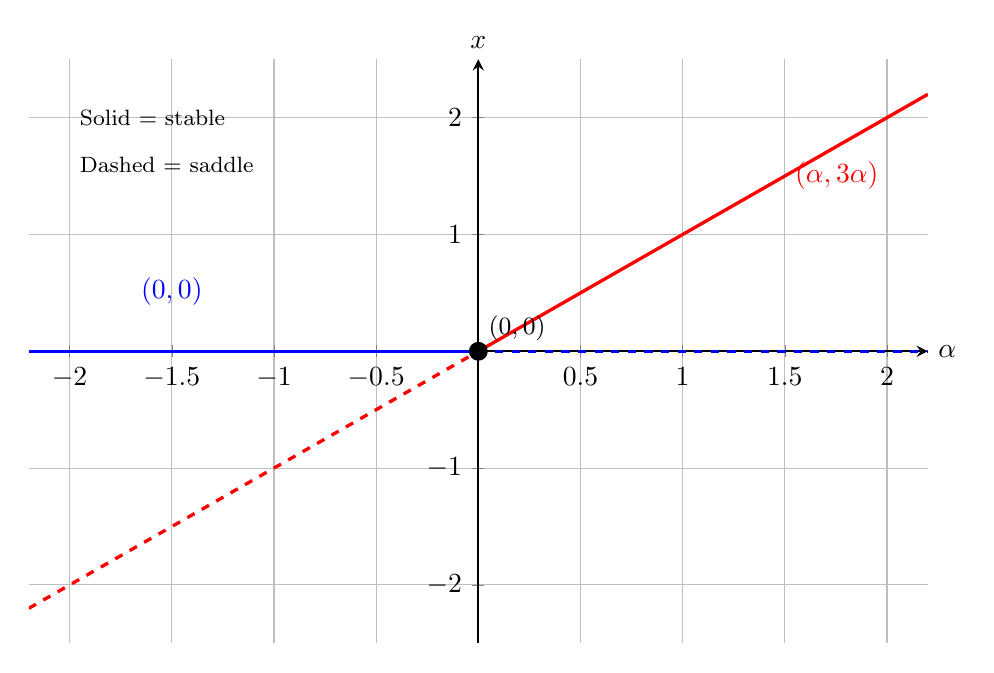
\begin{tikzpicture}
\begin{axis}[
    width=13cm,
    height=9cm,
    xlabel={$\alpha$},
    ylabel={$x$},
    xmin=-2.2, xmax=2.2,
    ymin=-2.5, ymax=2.5,
    grid=major,
    axis lines=middle,
    thick,
    every axis x label/.style={at={(current axis.right of origin)},anchor=west},
    every axis y label/.style={at={(current axis.above origin)},anchor=south}
]

% Branch 1: x = 0 stable (alpha < 0)
\addplot[blue, very thick, solid, domain=-2.2:0] {0};

% Branch 1: x = 0 unstable (alpha > 0)
\addplot[blue, very thick, dashed, domain=0:2.2] {0};

% Branch 2: x = alpha unstable (alpha < 0)
\addplot[red, very thick, dashed, domain=-2.2:0] {x};

% Branch 2: x = alpha stable (alpha > 0)
\addplot[red, very thick, solid, domain=0:2.2] {x};

% Bifurcation point
\addplot[mark=*, mark size=3pt, black, only marks] coordinates {(0, 0)};
\node[above right, font=\small] at (axis cs:0,0) {$(0, 0)$};

% Labels
\node[blue, anchor=south] at (axis cs:-1.5,0.3) {$(0,0)$};
\node[red, anchor=west] at (axis cs:1.5,1.5) {$(\alpha, 3\alpha)$};
\node[anchor=west, font=\footnotesize] at (axis cs:-2,2) {Solid = stable};
\node[anchor=west, font=\footnotesize] at (axis cs:-2,1.6) {Dashed = saddle};

\end{axis}
\end{tikzpicture}
\end{center}

\subsection*{XYZ Analysis of $(\alpha, x)$ Diagram}

\begin{itemize}[leftmargin=*]
\item \stage{STAGE X (What the diagram shows):} Two straight lines crossing at the origin. Horizontal line (pinned equilibrium) and diagonal line (moving equilibrium) exchange line styles at the crossing point.

\item \stage{STAGE Y (Why this structure):}
\begin{itemize}
\item The horizontal line $x = 0$ reflects that origin is always an equilibrium
\item The diagonal line $x = \alpha$ shows the moving equilibrium's $x$-coordinate equals the parameter value
\item They intersect at $\alpha = 0$ where both have $x = 0$ (collision point)
\item The line style swap (solid $\leftrightarrow$ dashed) encodes the stability exchange
\end{itemize}
Unlike a fold where branches meet in a parabola and terminate, here branches continue through each other as straight lines - the transcritical signature of "passing through" rather than "colliding and annihilating."

\item \stage{STAGE Z (What this tells us):} Reading left to right as $\alpha$ increases:
\begin{itemize}
\item Far left ($\alpha \ll 0$): stable equilibrium at origin, saddle far in third quadrant
\item Approaching zero: saddle moves toward origin along $y = 3x$ line
\item At zero: equilibria merge, both neutral
\item Past zero: origin becomes saddle, stable equilibrium moves into first quadrant
\item Far right ($\alpha \gg 0$): saddle at origin, stable equilibrium far in first quadrant
\end{itemize}
The system's attractor "jumps" from origin to the first quadrant as $\alpha$ crosses zero.
\end{itemize}

\vspace{10pt}
\hrule
\vspace{10pt}

\section{Step 8: Bifurcation Diagram ($\alpha$ vs $y$)}

\subsection*{Equilibrium branches in $(\alpha, y)$ space}

\textbf{Branch 1: Origin equilibrium}
\[
y = 0 \quad \text{for all } \alpha
\]
\begin{itemize}
\item Stable for $\alpha < 0$ (solid line)
\item Unstable (saddle) for $\alpha > 0$ (dashed line)
\end{itemize}

\textbf{Branch 2: Moving equilibrium}
\[
y = 3\alpha \quad \text{(diagonal line through origin, slope = 3)}
\]
\begin{itemize}
\item Unstable (saddle) for $\alpha < 0$ (dashed line)
\item Stable for $\alpha > 0$ (solid line)
\end{itemize}

\subsection*{Bifurcation diagram: $\alpha$ vs $y$}

\begin{center}
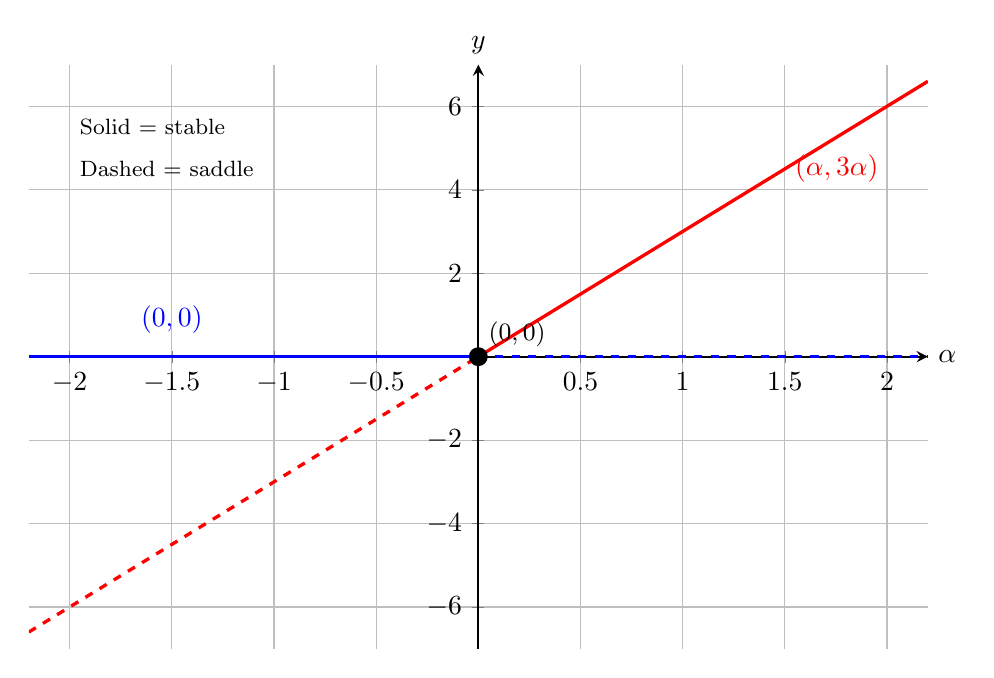
\begin{tikzpicture}
\begin{axis}[
    width=13cm,
    height=9cm,
    xlabel={$\alpha$},
    ylabel={$y$},
    xmin=-2.2, xmax=2.2,
    ymin=-7, ymax=7,
    grid=major,
    axis lines=middle,
    thick,
    every axis x label/.style={at={(current axis.right of origin)},anchor=west},
    every axis y label/.style={at={(current axis.above origin)},anchor=south}
]

% Branch 1: y = 0 stable (alpha < 0)
\addplot[blue, very thick, solid, domain=-2.2:0] {0};

% Branch 1: y = 0 unstable (alpha > 0)
\addplot[blue, very thick, dashed, domain=0:2.2] {0};

% Branch 2: y = 3*alpha unstable (alpha < 0)
\addplot[red, very thick, dashed, domain=-2.2:0] {3*x};

% Branch 2: y = 3*alpha stable (alpha > 0)
\addplot[red, very thick, solid, domain=0:2.2] {3*x};

% Bifurcation point
\addplot[mark=*, mark size=3pt, black, only marks] coordinates {(0, 0)};
\node[above right, font=\small] at (axis cs:0,0) {$(0, 0)$};

% Labels
\node[blue, anchor=south] at (axis cs:-1.5,0.3) {$(0,0)$};
\node[red, anchor=west] at (axis cs:1.5,4.5) {$(\alpha, 3\alpha)$};
\node[anchor=west, font=\footnotesize] at (axis cs:-2,5.5) {Solid = stable};
\node[anchor=west, font=\footnotesize] at (axis cs:-2,4.5) {Dashed = saddle};

\end{axis}
\end{tikzpicture}
\end{center}

\subsection*{Comparison of diagrams}

\begin{center}
\begin{tabular}{|l|c|c|}
\hline
\textbf{Feature} & \textbf{$\alpha$ vs $x$} & \textbf{$\alpha$ vs $y$} \\
\hline
Branch 1 (origin) & $x = 0$ (horizontal) & $y = 0$ (horizontal) \\
Branch 2 (moving) & $x = \alpha$ (slope 1) & $y = 3\alpha$ (slope 3) \\
Qualitative structure & Same & Same \\
Only difference & Scale of diagonal & Scale of diagonal \\
\hline
\end{tabular}
\end{center}

\subsection*{XYZ Analysis of $(\alpha, y)$ Diagram}

\begin{itemize}[leftmargin=*]
\item \stage{STAGE X (What changes):} The diagram looks similar but the moving equilibrium branch is steeper: slope 3 instead of 1. The stability patterns are identical.

\item \stage{STAGE Y (Why the difference):} Since the equilibrium coordinates are related by $y = 3x$, when we plot $y$ instead of $x$, we're simply rescaling the vertical axis by factor 3. The moving equilibrium has:
\begin{itemize}
\item $x$-coordinate: $\alpha$ (gives slope 1 in $\alpha$-$x$ plot)
\item $y$-coordinate: $3\alpha$ (gives slope 3 in $\alpha$-$y$ plot)
\end{itemize}
The constraint $y = 3x$ means the equilibria lie on a line in the $(x,y)$ phase plane. Projecting this line onto either coordinate axis gives the bifurcation diagram branches.

\item \stage{STAGE Z (What's invariant):} The qualitative bifurcation structure is independent of which coordinate we plot:
\begin{itemize}
\item Two straight lines crossing at origin
\item One horizontal (pinned equilibrium)
\item One diagonal (moving equilibrium)
\item Stability exchange at crossing
\end{itemize}
The choice of coordinate only affects quantitative details (slopes), not the bifurcation type or stability pattern. This reflects that bifurcations are coordinate-invariant phenomena - they're about the system's dynamics, not our choice of variables.
\end{itemize}

\vspace{10pt}
\hrule
\vspace{10pt}

\section{Step 9: Phase Portraits}

\subsection*{Three scenarios}

\begin{center}
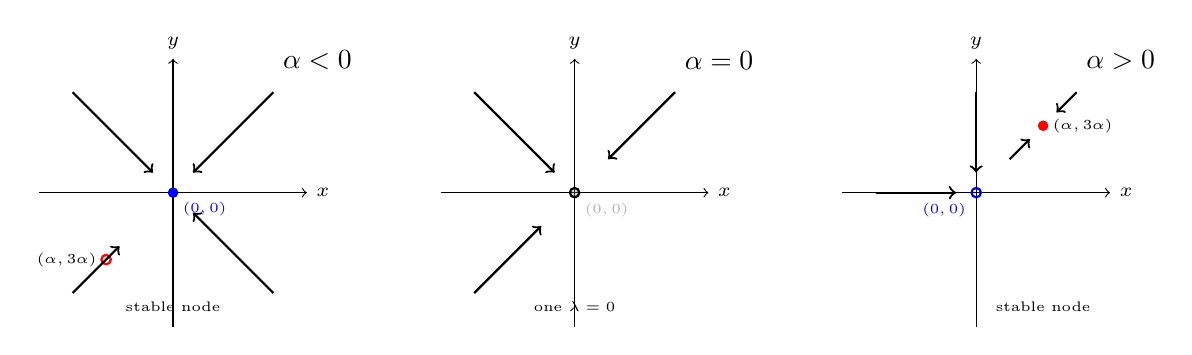
\begin{tikzpicture}[scale=0.85]
% alpha < 0
\begin{scope}
\draw[->] (-2,0) -- (2,0) node[right, font=\scriptsize] {$x$};
\draw[->] (0,-2) -- (0,2) node[above, font=\scriptsize] {$y$};
\node[above right] at (1.5,1.7) {$\alpha < 0$};
% Stable node at origin
\filldraw[blue] (0,0) circle (2pt) node[below right, font=\tiny] {$(0,0)$};
% Saddle in third quadrant
\draw[red, thick] (-1,-3*1/3) circle (2pt);
\node[font=\tiny, left] at (-1,-1) {$(\alpha, 3\alpha)$};
% Schematic flows
\draw[->, thick] (-1.5,-1.5) -- (-0.8,-0.8);
\draw[->, thick] (-1.5,1.5) -- (-0.3,0.3);
\draw[->, thick] (1.5,-1.5) -- (0.3,-0.3);
\draw[->, thick] (1.5,1.5) -- (0.3,0.3);
\node[font=\tiny] at (0,-1.7) {stable node};
\end{scope}

% alpha = 0
\begin{scope}[shift={(6,0)}]
\draw[->] (-2,0) -- (2,0) node[right, font=\scriptsize] {$x$};
\draw[->] (0,-2) -- (0,2) node[above, font=\scriptsize] {$y$};
\node[above right] at (1.5,1.7) {$\alpha = 0$};
% Degenerate equilibrium
\draw[black, thick, fill=gray, fill opacity=0.3] (0,0) circle (2pt) node[below right, font=\tiny] {$(0,0)$};
% Flows
\draw[->, thick] (-1.5,-1.5) -- (-0.5,-0.5);
\draw[->, thick] (-1.5,1.5) -- (-0.3,0.3);
\draw[->, thick] (1.5,1.5) -- (0.5,0.5);
\node[font=\tiny] at (0,-1.7) {one $\lambda = 0$};
\end{scope}

% alpha > 0
\begin{scope}[shift={(12,0)}]
\draw[->] (-2,0) -- (2,0) node[right, font=\scriptsize] {$x$};
\draw[->] (0,-2) -- (0,2) node[above, font=\scriptsize] {$y$};
\node[above right] at (1.5,1.7) {$\alpha > 0$};
% Saddle at origin
\draw[blue, thick] (0,0) circle (2pt) node[below left, font=\tiny] {$(0,0)$};
% Stable node in first quadrant
\filldraw[red] (1,1) circle (2pt);
\node[font=\tiny, right] at (1,1) {$(\alpha, 3\alpha)$};
% Schematic flows
\draw[->, thick] (-1.5,0) -- (-0.3,0);
\draw[->, thick] (0,1.5) -- (0,0.3);
\draw[->, thick] (1.5,1.5) -- (1.2,1.2);
\draw[->, thick] (0.5,0.5) -- (0.8,0.8);
\node[font=\tiny] at (1,-1.7) {stable node};
\end{scope}
\end{tikzpicture}
\end{center}

\textit{Notation: Filled circle = stable node, hollow circle = saddle}

\subsection*{XYZ Analysis of Phase Portrait Evolution}

\begin{itemize}[leftmargin=*]
\item \stage{STAGE X (What we see):} The stable attractor moves from origin to first quadrant as $\alpha$ increases through zero. The saddle point correspondingly moves from third quadrant to origin.

\item \stage{STAGE Y (Why these flows):} The flow directions are determined by the vector field:
\begin{itemize}
\item \textbf{For $\alpha < 0$}: Origin is stable node - all nearby trajectories flow inward (both eigenvalues negative). The saddle at $(\alpha, 3\alpha)$ has one stable direction (along eigenvector) and one unstable direction.
\item \textbf{For $\alpha = 0$}: One eigenvalue is zero at origin, creating a line of equilibria in that eigenvalue's direction (actually just one degenerate point here, but effectively neutral in one direction).
\item \textbf{For $\alpha > 0$}: Origin is saddle - trajectories approach along stable manifold but are repelled along unstable manifold. The equilibrium at $(\alpha, 3\alpha)$ is now the stable node, attracting nearby trajectories.
\end{itemize}

\item \stage{STAGE Z (What this means globally):} The basin of attraction fundamentally changes:
\begin{itemize}
\item Before bifurcation: Most trajectories near origin are attracted to $(0,0)$
\item After bifurcation: Most trajectories near origin are attracted to $(\alpha, 3\alpha)$ in first quadrant
\end{itemize}
The saddle at origin post-bifurcation acts as a "separatrix" - its stable manifold divides phase space into regions flowing to different fates. This is a qualitative change in global dynamics, not just local stability.
\end{itemize}

\vspace{10pt}
\hrule
\vspace{10pt}

\section{Summary}

\subsection*{Part (a): Equilibria and Stability}

\textbf{Equilibrium 1: $(0, 0)$}
\begin{itemize}
\item Always exists (pinned)
\item Stable node for $-9/4 < \alpha < 0$
\item Neutral for $\alpha = 0$ (eigenvalues: $0, -3$)
\item Saddle for $0 < \alpha < 9/4$
\end{itemize}

\textbf{Equilibrium 2: $(\alpha, 3\alpha)$}
\begin{itemize}
\item Exists for $\alpha \neq 0$
\item Saddle for $-9/4 < \alpha < 0$
\item Coincides with origin at $\alpha = 0$
\item Stable node for $0 < \alpha < 9/4$
\end{itemize}

\subsection*{Part (b): Bifurcation at $\alpha = 0$}

\[
\boxed{\text{TRANSCRITICAL BIFURCATION}}
\]

\textbf{Characteristics:}
\begin{itemize}
\item Pinned equilibrium at origin passes through by moving equilibrium
\item Equilibria exchange stability (stable node $\leftrightarrow$ saddle)
\item One eigenvalue crosses zero
\item No creation/destruction of equilibria
\end{itemize}

\subsection*{Part (c): Bifurcation Diagrams}

\textbf{$\alpha$ vs $x$ diagram:}
\begin{itemize}
\item Horizontal line: $x = 0$ (origin)
\item Diagonal line: $x = \alpha$ (slope 1)
\item Cross at $(\alpha, x) = (0, 0)$
\item Stability exchange at crossing
\end{itemize}

\textbf{$\alpha$ vs $y$ diagram:}
\begin{itemize}
\item Horizontal line: $y = 0$ (origin)
\item Diagonal line: $y = 3\alpha$ (slope 3)
\item Cross at $(\alpha, y) = (0, 0)$
\item Same qualitative structure, steeper slope
\end{itemize}

\textbf{Key insight:} Both diagrams show the same transcritical structure - two straight lines crossing with stability exchange. Only quantitative difference is the slope of the moving equilibrium branch (factor of 3 from $y = 3x$ constraint).

\end{document}
